\documentclass[12pt]{beamer}
\usetheme{Boadilla}
\usepackage{booktabs}
\usepackage{enumitem}
\usepackage{tikz}

\newcommand{\E}{\mathbb{E}}
\usefonttheme{professionalfonts}
\usepackage{pgfplots}
\renewcommand{\arraystretch}{1.25}
\usetikzlibrary{trees}
\title[ECON2843]{Lecture 12}
\subtitle{Part 3 Estimation and Hypothesis Test}
\date{}
\usepackage{amsmath,amssymb,mathtools,wasysym}
\begin{document}
	\begin{frame}
		\titlepage
	\end{frame}
	\begin{frame}
		\vspace{1cm}
		\centering
		{\color{blue}\large Estimation}
	\end{frame}
	\begin{frame}
		\frametitle{I Have a Problem...}
		
		\begin{itemize}[label={\color{blue}$\blacktriangleright$}]
			\item I ask myself at night, "Am I smarter than the average person?"
			\vspace{1cm}
			\item Step 1: Establish a variable of interest, such as IQ.
			\vspace{1cm}
			\item Step 2: Compare my IQ to a benchmark (population mean IQ).
		\end{itemize}
		
	\end{frame}
	\begin{frame}
		\frametitle{I Have a Problem...}
		
		\begin{itemize}[label={\color{blue}$\blacktriangleright$}]
			\item Randomly select a representative sample from the population.
			\vspace{1cm}
			\item Compare my IQ to the mean IQ of the sample.
			\vspace{1cm}
			\item So we are using a sample statistic (sample mean IQ) to estimate a population parameter (population mean IQ).
		\end{itemize}
		
	\end{frame}
\begin{frame}
	\frametitle{Sample Statistics as Estimators}
	
	\begin{itemize}[label={\color{blue}$\blacktriangleright$}]
		\item What did we see last topic?
		\item On average, the sample mean is approximately equal to the population mean.
		\begin{itemize}[label={\color{blue}$\blacktriangleright$}]
			\item The expected value of the sample mean was equal to the population mean, i.e., $E(\bar{X}) = \mu$.
		\end{itemize}
		\item As the sample size increased, the sample mean was much closer to the population mean.
		\begin{itemize}[label={\color{blue}$\blacktriangleright$}]
			\item The variance of the sample mean decreased as the sample size increased, i.e., $V(\bar{X}) = \frac{\sigma^2}{n}$.
		\end{itemize}
	\end{itemize}
	
\end{frame}
	\begin{frame}
	\frametitle{Two Types of Estimators}
	
	\begin{itemize}[label={\color{blue}$\blacktriangleright$}]
		\item {\bf Point estimator:} Draws inferences about a population by using a single value, calculated from a sample, to estimate an unknown population parameter.
		\item {\bf Interval estimator:} Draws inferences about a population by using an interval or range of values,calculated from a sample, to estimate an unknown population parameter.
	\end{itemize}
	
\end{frame}

\begin{frame}
	\frametitle{Point Estimators}
	
	\begin{itemize}[label={\color{blue}$\blacktriangleright$}]
		\item We have already seen examples of point estimators, e.g., $\bar{X}$ for $\mu$ and $s^2$ for $\sigma^2$.
		
		\item But there are many different sample statistics that we could use to estimate any particular population parameter.
		
		\item For example, we could also use the \textit{sample median} to estimate $\mu$.
		
		\item Given a population parameter, how can we choose which sample statistic to use as an estimator?
	\end{itemize}
	
\end{frame}
\begin{frame}
	\frametitle{Bias of a Point Estimator}
	
	\begin{itemize}[label={\color{blue}$\blacktriangleright$}]
		\item Let $\theta$ be some population parameter and let $\hat{\theta}$ denote a point estimator of $\theta$.
		
		\item The \textbf{bias} of a point estimator is defined to be:
		
		\[ B(\hat{\theta}) = E(\hat{\theta}) - \theta \]
		
		\item A point estimator is \textbf{unbiased} if $B(\hat{\theta}) = 0$, i.e., if $E(\hat{\theta}) = \theta$.
	\end{itemize}
	
\end{frame}
\begin{frame}
	\frametitle{Example of a Biased Point Estimator}
	
	\begin{itemize}[label={\color{blue}$\blacktriangleright$}]
		\item Consider estimating the population variance $\sigma^2$ using the sample variance:
		
		\[
		S^2 = \frac{1}{n} \sum_{i=1}^n (X_i - \bar{X})^2
		\]
		
		\item This estimator is biased because:
		
		\[
		E(S^2) = \frac{n-1}{n} \sigma^2 \neq \sigma^2
		\]
		
	\end{itemize}
	
	\end{frame}
\begin{frame}
	\frametitle{Bias of a Point Estimator}
	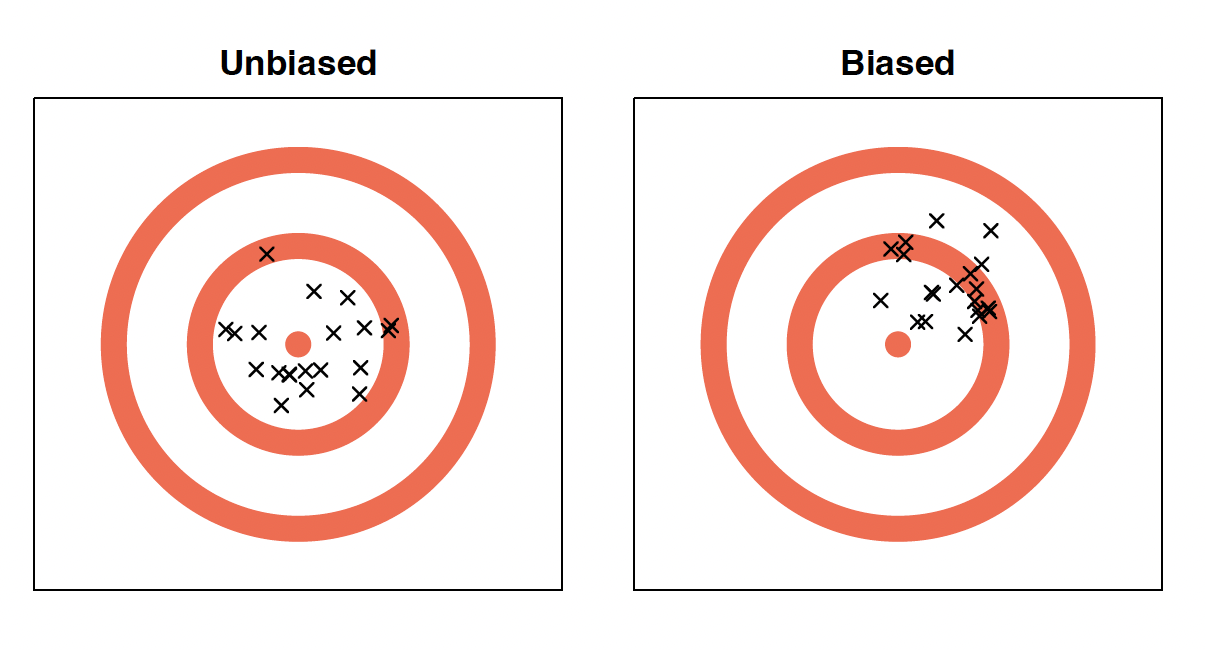
\includegraphics[width=12cm]{biase.png}
\end{frame}
\begin{frame}
	\frametitle{A Real-world Example}
	
	\begin{itemize}[label={\color{blue}$\blacktriangleright$}]
		\item Scenario: Estimating average fish length in a lake
		
		\item Biased method: Using a net with 10cm gaps between threads
		
		\item This method is biased because:
		\begin{itemize}
			\item Fish smaller than 10cm escape through the gaps
			\item Estimated average length will be higher than true average
		\end{itemize}
		
		\item If true average length is 12cm:
		\begin{itemize}
			\item Biased estimate might be 15cm
			\item Bias = 15cm - 12cm = 3cm (overestimation)
		\end{itemize}
		
		\item Unbiased alternative: Use a net with very small gaps or a variety of gap sizes
	\end{itemize}
	
\end{frame}
\begin{frame}
	\frametitle{Bias of a Point Estimator}
	
	\begin{itemize}[label={\color{blue}$\blacktriangleright$}]
		\item Unbiasedness is a desirable quality of a point estimator.
		
		\item We know that $E(\bar{X}) = \mu$, so $\bar{X}$ is an unbiased estimator of $\mu$.
		
		\item We have shown that $s^2= \frac{1}{n-1} \sum_{i=1}^n (X_i - \bar{X})^2$ is an unbiased estimator of $\sigma^2$.
	\end{itemize}
	
\end{frame}

\begin{frame}
	\frametitle{Variance of a Point Estimator}
	
	\begin{itemize}[label={\color{blue}$\blacktriangleright$}]
		\item If $\hat{\theta}$ is a point estimator of $\theta$, the \textbf{variance} of $\hat{\theta}$ is:
		
		\[
		V(\hat{\theta}) = E\left(\left(\hat{\theta} - E(\hat{\theta})\right)^2\right)
		\]
		\[
		= E(\hat{\theta}^2) - \left(E(\hat{\theta})\right)^2
		\]
		
		\item We would like our estimators to have low variance.
	\end{itemize}
	
\end{frame}
\begin{frame}
	\frametitle{Variance of a Point Estimator}
	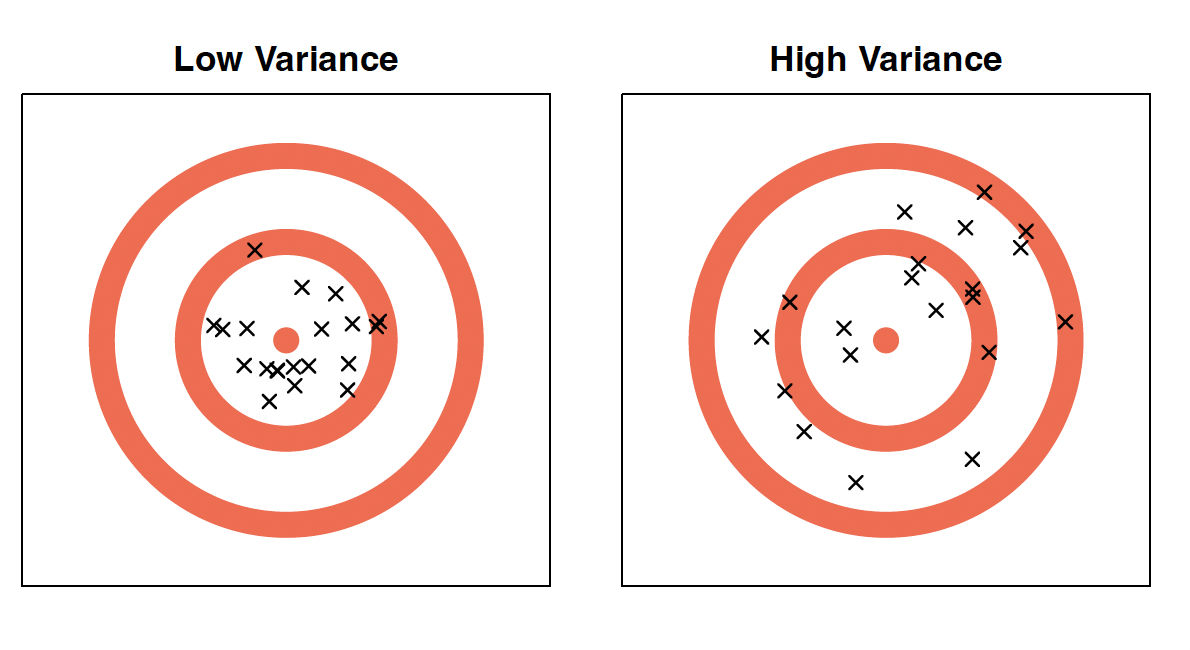
\includegraphics[width=12cm]{variance.png}
\end{frame}


\begin{frame}
	\frametitle{Low vs High Variance Estimators}
	
	\begin{itemize}[label={\color{blue}$\blacktriangleright$}]
		\item If you want to estimate average daily sales in a coffee shop
		
		\item Low Variance Estimator: Average sales over 30 days
		\begin{itemize}
			\item Example results: \$985, \$1010, \$995 (multiple samples)
			\item Low spread around true value
		\end{itemize}
		
		\item High Variance Estimator: Sales from a single randomly chosen day
		\begin{itemize}
			\item Example results: \$1200, \$800, \$1100 (multiple samples)
			\item High spread around true value
		\end{itemize}
		
		\item Implications:
		\begin{itemize}
			\item Low variance: More reliable estimates
			\item High variance: Less reliable, more prone to extreme values
		\end{itemize}
	\end{itemize}
	
\end{frame}
\begin{frame}
	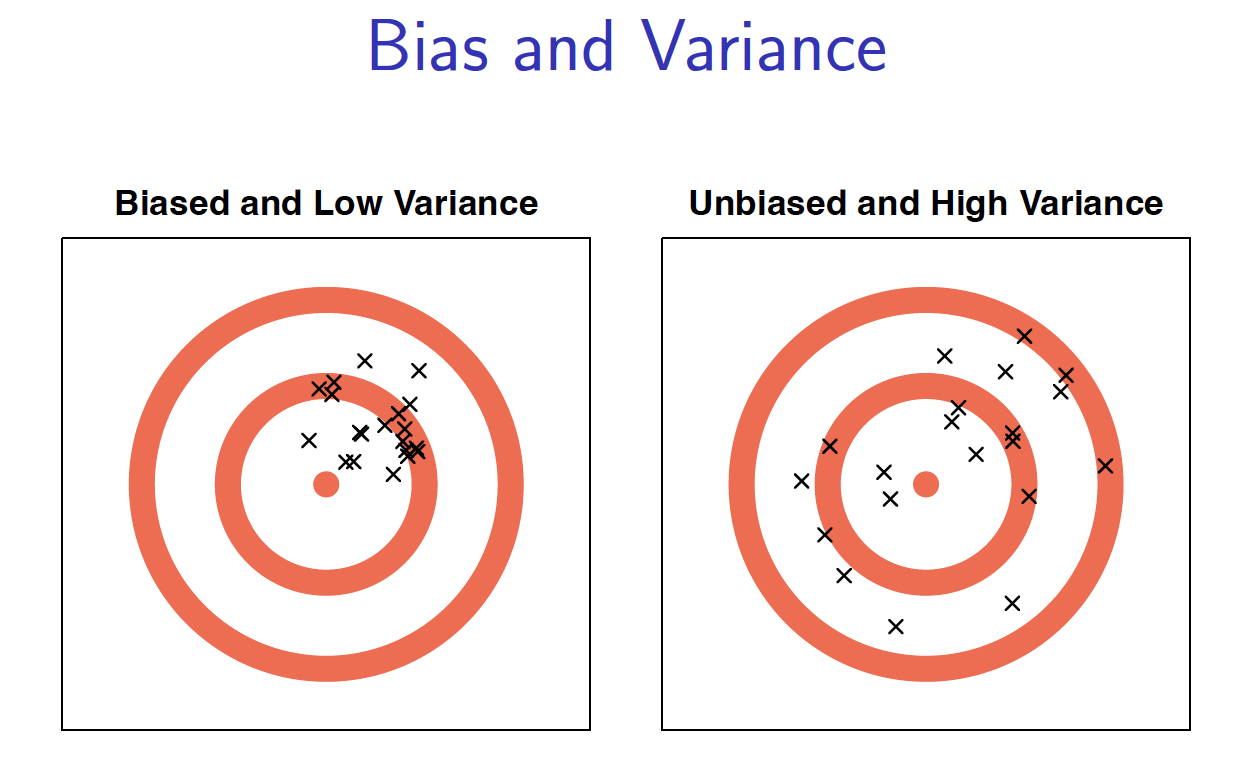
\includegraphics[width=12cm]{bv.png}
\end{frame}
\begin{frame}
\frametitle{Trade-off}

\begin{itemize}[label={\color{blue}$\blacktriangleright$}]
\item There is often a trade-off between minimizing bias and minimizing variance. Why the trade-off?
\begin{itemize}[label={\color{blue}$\blacktriangleright$}]
	\item Reducing bias often increases complexity of the estimator
	\item More complex estimators tend to have higher variance
\end{itemize}
	\end{itemize}

\end{frame}
\begin{frame}
	\frametitle{Mean Squared Error of a Point Estimator}
	
	\begin{itemize}[label={\color{blue}$\blacktriangleright$}]
		
		\item If $\hat{\theta}$ is a point estimator of $\theta$, the \textbf{mean squared error} of $\hat{\theta}$ is defined to be:
		
		\[
		MSE(\hat{\theta}) = E\left(\left(\hat{\theta} - \theta\right)^2\right)
		\]
		\[
		= V(\hat{\theta}) + \left(B(\hat{\theta})\right)^2
		\]
		
		\item MSE can be useful for comparing point estimators.
		\item Mean Squared Error (MSE) = Variance + Bias$^2$
	\end{itemize}
	
\end{frame}

%\begin{frame}
%	\frametitle{\textcolor{blue}{Understanding Mean Squared Error}}
%	
%	\begin{itemize}[label={\color{blue}$\blacktriangleright$}]
%		
%		\item Imagine a meteorologist predicting daily low temperatures for a week.
%		
%		\item Actual vs. Predicted Temperatures (°F):
%		
%	\end{itemize}
%	\centering
%\begin{tabular}{c|c|c|c}
%	Day & Actual & Predicted & Error \\
%	\hline
%	1 & 25 & 24 & -1 \\
%	2 & 28 & 30 & +2 \\
%	3 & 27 & 26 & -1 \\
%	4 & 26 & 28 & +2 \\
%	5 & 29 & 27 & -2 \\
%\end{tabular}
%\end{frame}
%\begin{frame}
%	\frametitle{\textcolor{blue}{Understanding Mean Squared Error}}
%	
%	\begin{itemize}[label={\color{blue}$\blacktriangleright$}]
%		\item \textbf{Calculating MSE:}
%		\begin{align*}
%			\text{MSE} &= \frac{1}{n} \sum_{i=1}^n (y_i - \hat{y}_i)^2 \\
%			&= \frac{1}{5} [((-1)^2 + 2^2 + (-1)^2 + 2^2 + (-2)^2] \\
%			&= \frac{1}{5} [1 + 4 + 1 + 4 + 4] = \frac{14}{5} = 2.8
%		\end{align*}
%		
%		\item MSE of 2.8$°F^2$ indicates the average squared deviation of predictions.
%		
%		\item Lower MSE suggests more accurate predictions.
%	\end{itemize}
%	
%\end{frame}

\begin{frame}
	\frametitle{\textcolor{blue}{Mean Squared Error: Understanding the Bias-Variance Trade-off}}
	
	\begin{itemize}[label={\color{blue}$\blacktriangleright$}]
		\item MSE can be decomposed into two components:
		\begin{equation*}
			\text{MSE} = \text{Bias}^2 + \text{Variance}
		\end{equation*}
		
		\item \textbf{Bias}: How far off our predictions are from the true value.
		\begin{itemize}
			\item High bias: Underfitting (oversimplified model)
			\item Low bias: Captures underlying pattern well
		\end{itemize}
		
		\item \textbf{Variance}: How much our predictions vary for different samples.
		\begin{itemize}
			\item High variance: Overfitting (too sensitive to noise in data)
			\item Low variance: More stable predictions across samples
		\end{itemize}
			\end{itemize}
		
		
	\end{frame}
\begin{frame}
	\frametitle{\textcolor{blue}{Mean Squared Error: Understanding the Bias-Variance Trade-off}}
	
	\begin{itemize}[label={\color{blue}$\blacktriangleright$}]
		\item \textbf{The Trade-off}:
		\begin{itemize}
			\item As model complexity increases: Bias $\downarrow$, Variance $\uparrow$
			\item As model complexity decreases: Bias $\uparrow$, Variance $\downarrow$
		\end{itemize}
		
		\item Goal: Find the sweet spot that minimizes total error (MSE)
	\end{itemize}
	

\end{frame}

\begin{frame}
	\frametitle{\textcolor{blue}{Bias-Variance Trade-off: House Price Prediction}}
	
	\begin{itemize}[label={\color{blue}$\blacktriangleright$}]
		\item Predicting house prices based on square footage
		
		\item Data(our sample): 100 houses with their prices and square footage
		
		\item We use two ways to estimate
		\begin{itemize}[label={\color{blue}$\blacktriangleright$}]
			\item Linear: Price = a $\times$ (Square Footage) + b
			\item Quadratic: Price = a $\times$ (Square Footage)$^2$ + b $\times$ (Square Footage) + c
		\end{itemize}
	\end{itemize}

\end{frame}
\begin{frame}
	\frametitle{\textcolor{blue}{Bias-Variance Trade-off: House Price Prediction}}
	
	\begin{itemize}[label={\color{blue}$\blacktriangleright$}]
		\item \textbf{Results:}
		\begin{tabular}{l|c|c|c}
			Model & Bias & Variance & MSE \\
			\hline
			Linear & High & Low & 10,000 \\
			Quadratic & Low & High & 8,000 \\
		\end{tabular}
		
		\item \textbf{Interpretation:}
		\begin{itemize}[label={\color{blue}$\blacktriangleright$}]
			\item Linear: Underfits (high bias), but consistent (low variance)
			\item Quadratic: Balances bias and variance, lowest overall error
		\end{itemize}
		
		\item The quadratic model finds the "sweet spot" in the bias-variance trade-off for this dataset.
	\end{itemize}
$$\text{MSE} = \frac{1}{n} \sum_{i=1}^n (\text{Price}_i - \hat{\text{Price}}_i)^2,\quad n=100 {\text{ here}}$$
	
\end{frame}

\begin{frame}
	\frametitle{Why We Need MSE: For Consistency!}
	
	\begin{itemize}[label={\color{blue}$\blacktriangleright$}]
		\item An estimator is said to be \emph{consistent} if it approaches (i.e., gets closer to) the population parameter as the sample size increases.
		\item In other words...
		
		\item We can use the mean squared error to measure closeness.
		
		\item Let $\hat{\theta}$ be a point estimator of $\theta$. If $MSE(\hat{\theta}) \to 0$ as $n \to \infty$, then $\hat{\theta}$ is a \textbf{consistent} estimator of $\theta$.
		\vspace{0.5cm}
		\item Now you should be able to tell me what is a point estimator: Mean, Median, Mode, Variance?
	\end{itemize}
	
\end{frame}

\begin{frame}
	\frametitle{Consistency: Examples}
	
	\begin{itemize}[label={\color{blue}$\blacktriangleright$}]
		\item Is $\bar{X}$ a consistent estimator of $\mu$? Yes!
		\vspace{1cm}
		\begin{itemize}[label={\color{blue}$\blacktriangleright$}]
			\item We know that $E(\bar{X}) = \mu$ and $V(\bar{X}) = \frac{\sigma^2}{n}$.
			\item[] $\therefore MSE(\bar{X}) = \frac{\sigma^2}{n} + 0^2 \to 0 \quad \text{as} \quad n \to \infty$
		\end{itemize}
	\end{itemize}

\end{frame}
\begin{frame}
	\frametitle{Recall the Sample Proportion We Learned}
	
	\begin{itemize}[label={\color{blue}$\blacktriangleright$}]
		\item $X = \sum_{i=1}^n X_i$, where
		
		\[
		X_i = \begin{cases}
			1 & \text{person $i$ prefers Coke over Pepsi} \\
			0 & \text{otherwise}
		\end{cases}
		\]
		
		\item So $\hat{p}$ is just {\bf the sample mean} of a sample of independent Bernoulli random variables:
		
		\[
		\hat{p} = \frac{X}{n} = \frac{\sum_{i=1}^n X_i}{n}
		\]
	\end{itemize}
	
\end{frame}
\begin{frame}
	\frametitle{Consistency: Examples}
\begin{itemize}[label={\color{blue}$\blacktriangleright$}]
		\item Is the sample proportion, $\hat{p} = \frac{X}{n}$, a consistent estimator of $p$? Yes!
		\vspace{1cm}
		\begin{itemize}[label={\color{blue}$\blacktriangleright$}]
			\item Previously we showed that $E(\hat{p}) = p$ and $V(\hat{p}) = \frac{p(1-p)}{n}$.
			\item[] $\therefore MSE(\hat{p}) = \frac{p(1-p)}{n} + 0^2 \to 0 \quad \text{as} \quad n \to \infty$
		\end{itemize}
	\end{itemize}
	
\end{frame}

\begin{frame}{Is sample variance a consistent estimator for population variance?}
	$$s^2= \frac{1}{n-1} \sum_{i=1}^n (X_i - \bar{X})^2,\quad\sigma^2=\frac{1}{n} \sum_{i=1}^n(X_i-\mu)^2$$
	\begin{itemize}[label={\color{blue}$\blacktriangleright$}]
		\item We have proved unbiasedness of $s^2$.
		\item And we just proved, as $n \to \infty$:
		\begin{itemize}[label={\color{blue}$\blacktriangleright$}]
			\item $\bar{X} \to \mu$ (sample mean converges to population mean)
		\end{itemize}
		Recall that
		\begin{equation*}
			\text{MSE} = \text{Bias}^2 + \text{Variance}
		\end{equation*}
		\item For this question, we need to calculate the variance of sample variance!
	\end{itemize}
\end{frame}


\begin{frame}{Variance of the Sample Variance}
	
	The variance of \( S^2 \), by the shortcut formula $V(X)=\E(X^2)-\E(X^2)$, is:
	$$V(S^2) = \mathbb{E}[(S^2)^2] - (\mathbb{E}[S^2])^2= \mathbb{E}[(S^2)^2]-\sigma^4$$
	
	After expansion and using properties of expectations:
	\begin{equation*}
		\text{Var}(S^2) = \frac{\E(X_i^4)}{n}-\frac{\sigma^4(n-3)}{n(n-1)}\to0,\text{ as }n\to\infty 
	\end{equation*}
	
\end{frame}

\begin{frame}
	\frametitle{Relative Efficiency}
	
	\begin{itemize}[label={\color{blue}$\blacktriangleright$}]
		\item Let $\hat{\theta}_1$ and $\hat{\theta}_2$ be two \emph{unbiased} point estimators of $\theta$. The \textbf{relative efficiency} of $\hat{\theta}_1$ with respect to $\hat{\theta}_2$ is defined to be:
		
		\[
		\text{eff}(\hat{\theta}_1, \hat{\theta}_2) = \frac{V(\hat{\theta}_2)}{V(\hat{\theta}_1)}
		\]
		
		\item The unbiased estimator with the smaller variance is said to be \textbf{relatively more efficient}.
	\end{itemize}
	
\end{frame}
\begin{frame}
	\frametitle{Relative Efficiency}
	
	\begin{itemize}[label={\color{blue}$\blacktriangleright$}]
		\item For example, for a normal distribution, it can be shown that the sample median has expected value equal to $\mu$ and variance equal to $\frac{1.5708 \times \sigma^2}{n}$.
		
		\item[] $\therefore \text{eff}(\bar{X}, \text{Med}) = \frac{V(\text{Med})}{V(\bar{X})} = \frac{\frac{1.5708 \times \sigma^2}{n}}{\frac{\sigma^2}{n}} = 1.5708$
		
		\item Since $\text{eff}(\bar{X}, \text{Med}) > 1$, i.e., $V(\bar{X}) < V(\text{Med})$, $\bar{X}$ is relatively more efficient than the sample median for estimating $\mu$ in a normal distribution.
	\end{itemize}
	
\end{frame}

\begin{frame}
	\frametitle{Interval Estimators}
	
	\begin{itemize}[label={\color{blue}$\blacktriangleright$}]
		\item Why use interval estimators?
		\begin{itemize}[label={\color{blue}$\blacktriangleright$}]
			\item Point estimators will almost always be wrong.
			\item Difficult to tell how close a point estimator is to the parameter.
			\item Point estimators do not reflect the effects of larger sample sizes.
		\end{itemize}
		
		\item How do we construct an interval estimator?
		\begin{itemize}[label={\color{blue}$\blacktriangleright$}]
			\item Recall that sampling distributions gave us the distribution of an estimator (sample statistic).
			\item We will use \emph{probabilities} derived from the sampling distribution of the estimator to construct an interval estimator.
		\end{itemize}
	\end{itemize}
	
\end{frame}
\begin{frame}
	\frametitle{Estimating $\mu$ ($\sigma^2$ Known)}
	
	\begin{itemize}[label={\color{blue}$\blacktriangleright$}]
		\item To construct an interval estimator for $\mu$ based on $\bar{X}$ (when the population variance is known) we will use its sampling distribution via the Central Limit Theorem.
		
		\item Specifically, we know that the sample mean follows a normal distribution for large sample sizes.
		
		\item We will use the $z$-tables to determine the associated probabilities.
	\end{itemize}
	
\end{frame}

\begin{frame}
	\frametitle{Central Limit Theorem}
	
	\begin{itemize}[label={\color{blue}$\blacktriangleright$}]
		\item From the CLT, we know that for large $n$:
		
		\[
		\bar{X} \sim N\left(\mu, \frac{\sigma^2}{n}\right)
		\]
		
		\item And if we standardize, we get:
		
		\[
		Z = \frac{\bar{X} - \mu}{\frac{\sigma}{\sqrt{n}}} \sim N(0, 1)
		\]
	\end{itemize}
	
\end{frame}
\begin{frame}
	\frametitle{Standard Normal Distribution}
	$$P(-1.96<Z<1.96)=0.95$$
	\centering
	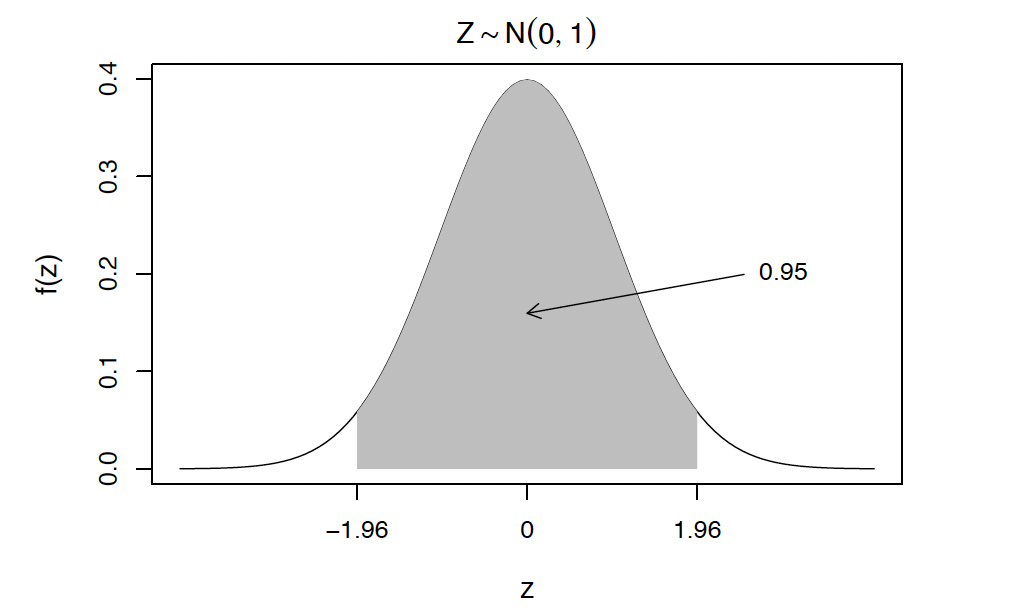
\includegraphics[width=10cm]{standard.png}
\end{frame}
\begin{frame}
	\frametitle{Standard Normal Distribution}
	\centering
	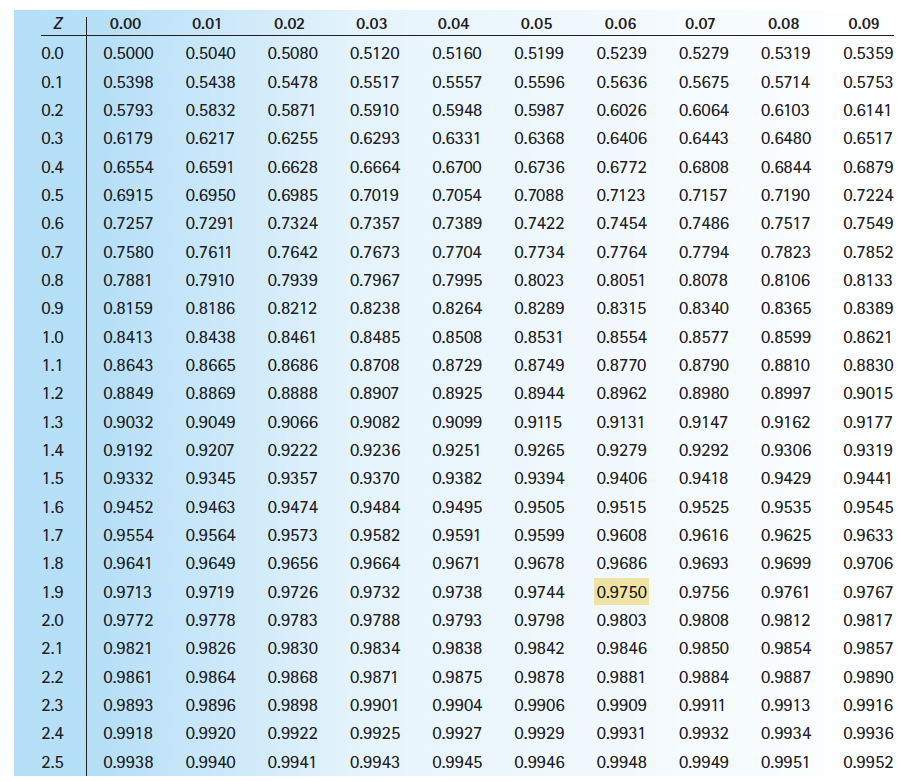
\includegraphics[width=9cm]{ztable.png}
\end{frame}
\begin{frame}
	\frametitle{Interval Estimator for $\mu$}
	
	\begin{align*}
		P(-1.96 < Z < 1.96) &= 0.95 \\[0.5em]
		P\left(-1.96 < \frac{\bar{X} - \mu}{\frac{\sigma}{\sqrt{n}}} < 1.96\right) &= 0.95 \\
		P\left(-1.96\frac{\sigma}{\sqrt{n}} < \bar{X} - \mu < 1.96\frac{\sigma}{\sqrt{n}}\right) &= 0.95 \\
		P\left(-1.96\frac{\sigma}{\sqrt{n}} - \bar{X} < -\mu < 1.96\frac{\sigma}{\sqrt{n}} - \bar{X}\right) &= 0.95 \\
		P\left(1.96\frac{\sigma}{\sqrt{n}} + \bar{X} > \mu > -1.96\frac{\sigma}{\sqrt{n}} + \bar{X}\right) &= 0.95 \\
		P\left(\bar{X} - 1.96\frac{\sigma}{\sqrt{n}} < \mu < \bar{X} + 1.96\frac{\sigma}{\sqrt{n}}\right) &= 0.95
	\end{align*}
	
\end{frame}
\begin{frame}
	\frametitle{95\% Confidence Interval for $\mu$}
	
	\begin{itemize}[label={\color{blue}$\blacktriangleright$}]
		\item So our interval estimator for $\mu$ when $\sigma^2$ is known is given by:
		
		\[
		\bar{X} \pm 1.96\frac{\sigma}{\sqrt{n}} = \left(\bar{X} - 1.96\frac{\sigma}{\sqrt{n}}, \bar{X} + 1.96\frac{\sigma}{\sqrt{n}}\right)
		\]
		
		\item This is called a 95\% \textbf{confidence interval} for $\mu$.
		
		\item What this means: In repeated sampling, 95\% of the intervals created in this way would contain $\mu$ and 5\% would not.
	\end{itemize}
	
	\end{frame}
	
	\begin{frame}
		\frametitle{95\% Confidence Interval for $\mu$}
		
		\[
		P\left(\bar{X} - 1.96\frac{\sigma}{\sqrt{n}} < \mu < \bar{X} + 1.96\frac{\sigma}{\sqrt{n}}\right) = 0.95
		\]
		
		\begin{itemize}[label={\color{blue}$\blacktriangleright$}]
			\item What made this a 95\% confidence interval?
		\end{itemize}
		
		\[
		\bar{X} \pm 1.96\frac{\sigma}{\sqrt{n}} = \left(\bar{X} - 1.96\frac{\sigma}{\sqrt{n}}, \bar{X} + 1.96\frac{\sigma}{\sqrt{n}}\right)
		\]
		
	\end{frame}
\end{document}